\graphicspath{{./lab02/Images/}}


\maketitlepage{App Development}{in Android Studio}{Lab 2: Threads}
\maketocpage

\section{Java Threads}
This section offers a brief introduction to threading in Java but anyone with prior knowledge is free to skip to the next section. The source code for all code examples is available \href{https://github.com/JonSteinn/AndroidDevelopment/tree/master/examples/lab2/javathreads}{here} and a programming session \href{https://www.youtube.com/watch?v=JqSdEsKneJc}{here}. The programming session is done in IntelliJ and there is a video of it being setup \href{https://youtu.be/JpKJMFytYTE}{here}

\begin{table}[H]
\center
\begin{tabular}{l|l}
method & functionality \\
\hline
\texttt{Thread(Runnable runnable)} & Creates a new thread \\
\texttt{void start()} & Causes this thread to begin execution \\
\texttt{void join()} & Makes the calling thread wait until this one dies. \\
\texttt{boolean isAlive()} & Returns true iff thread has started and is not dead \\
\texttt{String getName()} & Returns the thread's name
\end{tabular}
\caption{Parts of the Thread API}
\label{table:tapi}
\end{table}

Threads, in its simplest form, are a way to execute two (or more) blocks of code at the same time while sharing certain resources. Each thread executes a run method, line by line, and once started, we have limited control over the order of which thread is being executed\footnote{A context switch is when an operating system switches execution from one thread to another}. In the following we have three threads, the thread that starts the other two (the main thread) which will print \texttt{X} and \texttt{thread1} and \texttt{thread2}, printing \texttt{A} and \texttt{1} respectively. Running this program produces an nondeterministic output, in fact all possible permutations of \texttt{A}, \texttt{1} and \texttt{X} can be printed.
\begin{lstlisting}[style=A_Java]
public static void main(String[] args) {
    Thread thread1 = new Thread(() -> System.out.print("A"));
    Thread thread2 = new Thread(() -> System.out.print("1"));
    thread1.start();
    thread2.start();
    System.out.print("X");
}
\end{lstlisting}
One reason to use threads is to keep an UI from locking while a long task is happening in the background. Here we see a task being run in the background while the main thread keeps the user informed. A more familiar version of this idea is a spinning wheel for the user to look at while he waits.
\begin{lstlisting}[style=A_Java]
public class Main {
    public static void main(String[] args) {
        try {
            Thread carpenter = new Thread(() -> buildHouse(3));
            System.out.println("Ready to work");
            carpenter.start();
            while (true) {
                System.out.println("Work in progress...");
                carpenter.join(500); // wait 0.5s for thread to finish
                if (carpenter.isAlive()) continue;
                System.out.println("Work complete");
                break;
            }
        } catch (InterruptedException ex) {
            ex.printStackTrace();
        }
    }
    public static void buildHouse(int sec) {
        long timePoint = System.currentTimeMillis() + sec * 1000;
        while(System.currentTimeMillis() < timePoint); // loop for sec seconds
    }
}
\end{lstlisting}
A race conditions can occur when two threads access and edit the same resource in an unexpected order. Suppose thread A and B are both running and their job is to increment a shared variable X, which is set as 0. Thread A loads the value of X as 0 into registry when a context switch occurs and thread B loads the value of X into registry as 0 too, then B adds one and stores the value in X before another context switch when thread A does the same, both adding 1 to 0, so the variable ends up as 1, not 2. The part of the code where race conditions can occur is called a critical section. We must pay close attention to them when dealing with threads.\\

In the program below we start thousand threads that increment two variables which are initially equal and then check if they are still equal, upon which we increment a counter. A sequential run of such a program would always increment the variable one at a time, check if they are equal which they will always be and then increment the counter, resulting in him being 1000 at the end. What can happen here is that thread $i$ is running and has just incremented the variable \texttt{a} when a context switch occurs and thread $j$ starts to run which now increments \texttt{a} again and then \texttt{b} and when done, checks if they are equal which they are not since thread $i$ only incremented \texttt{a} so $j$ will not increment the counter variable. Of course we can get lucky and everything happens in the correct order, even most of the time, but a slim chance of a race condition is all that is needed to make an entire program ruined.  
\begin{lstlisting}[style=A_Java]
public class Main {
    private static int counter = 0, a = 0, b = 0;
    public static void main(String[] args) {
        try {
            Thread[] threads = new Thread[1000];
            for (int i = 0; i < threads.length; i++) {
                threads[i] = new Thread(() -> {
                    if (++a == ++b) counter++;
                });
                threads[i].start();
            }
            for (Thread t : threads) t.join();
            System.out.println(counter);
        } catch (InterruptedException e) {
            e.printStackTrace();
        }
    }
}
\end{lstlisting}
To deal with race conditions, we can identify the critical section and make sure that only one thread can operate there at any given time. That does however come at the cost of execution speed so we must place such lockouts wisely. When some thread arrives at a critical section, it should either be locked and make the thread wait or as soon as the thread 'steps in', the section should lock other threads out, until the current one is done. This can be done with the Java keyword \verb!synchronized!. Synchronized methods can only be run by one thread at a time. Synchronized can also be used on scopes. Another approach is to use a mutex. One can think of a mutex like a single key which you must acquire to reach a critical section but once used, no one else can use it until the current key user has returned it after leaving the critical section. In Java, mutexes are instances of the class \texttt{Semaphore}, a more general case of a mutex for arbitrary number of keys (even a negative amount!). Using a Semaphore initialized with a key count of 1, the following mutex will fix our race condition even though, locking the entire part of a thread does not make good use of them.
\begin{lstlisting}[style=A_Java]
threads[i] = new Thread(() -> {
  try {
    mutex.acquire();                    // Get the only key
    /* Critical section begins */
    if (++a == ++b) counter++;
    /* Critical section ends */
    mutex.release();                    // Give back the only key
  } catch (InterruptedException e) {
    e.printStackTrace();
  }
});
\end{lstlisting}
Using such locks brings about another problem. What if Thread $i$ is waiting on thread $j$ and thread $j$ is waiting on thread $i$? The waiting will go on forever and is called a deadlock. In the following code, suppose that the thread \texttt{t1} start and acquires \texttt{mutex1} but as soon as he has, a context switch occurs and the thread \texttt{t2} starts to run and acquires \texttt{mutex2}. Now it does not matter which thread is running, both mutexes are locked and both threads are unable to acquire the 'key'.
\begin{lstlisting}[style=A_Java]
public class Main {
    public static void main(String[] args) {
        Semaphore mutex1 = new Semaphore(1);
        Semaphore mutex2 = new Semaphore(1);
        Thread t1 = new Thread(() -> {
            try {
                mutex1.acquire();
                // Thread 1 stuck here
                mutex2.acquire();
                mutex1.release();
                mutex2.release();
            } catch (InterruptedException e) {
                e.printStackTrace();
            }
        });
        Thread t2 = new Thread(() -> {
            try {
                mutex2.acquire();
                // Thread 2 stuck here
                mutex1.acquire();
                mutex2.release();
                mutex1.release();
            } catch (InterruptedException e) {
                e.printStackTrace();
            }
        });
        t1.start();
        t2.start();
    }
}
\end{lstlisting}
Thread pools are used to gain more control over threads in Java. We can control the upper bound of how many threads are active at any given time from a pool. This is done with \texttt{Executor} and \texttt{ExecutorService}. Here we have a thread pool with a thread limit of five but 15 threads to start. As soon as 5 threads are already active, no more are added until at least one of them finishes.
\begin{lstlisting}[style=A_Java]
public static void main(String[] args) {
    ExecutorService executor = Executors.newFixedThreadPool(5);
    for (int i = 0; i < 15; i++) {
        executor.execute(() -> {
            try {
                System.out.println(Thread.currentThread().getName() + ": Hi");
                Thread.sleep(1000);
                System.out.println(Thread.currentThread().getName() + ": Bye");
            } catch (InterruptedException e) {
                e.printStackTrace();
            }/
        });
    }
    executor.shutdown();
}
\end{lstlisting}

\section{The Android UI thread}
Upon starting an Android app, a thread is created which will run our launcher activity and from there on, any component (which we will look at later). It also handles all events and interaction concerning the UI. No other threads should interact directly with the UI. This thread is called the main thread or the UI thread.\\

Suppose our app needs to run a long and expensive task, taking 10 seconds to execute. If we were to run that on the main thread, then it would not be able to listen for any events during the task and the UI would essentially be locked and eventually the operating system would warn the user that the app is not responding. To avoid this, all expensive tasks should be performed by new threads in the background of the main one. Tasks like calling a web service, downloading and many more.\\

Just as the UI thread should not run long tasks, the vice versa holds, that long task running threads should never update the UI. The two rules of thumb are
\begin{itemize}
\item \textbf{Never run a long task on the UI thread}
\item \textbf{Never update your UI from any thread other than the UI thread}
\end{itemize}

There are multiple Android specific ways to create and managing threads but we will only look at few here. Background tasks in Android can bring about some memory issues which we will address when looking at activities.

\section{Asynchronous tasks}
The abstract class \texttt{AsyncTask} provides an easy way to perform a background task which can talk to the UI thread. Asynchronous tasks are used for a short task required to run in a background thread, preferably not running longer than a few seconds. They are however bound to the lifetime of their activity.\\

The \texttt{AsyncTask} class has 3 generic types,
\begin{itemize}
\item \texttt{Params}. The type of parameter sent to task upon execution.
\item \texttt{Progress}. The type of progress unit published during task.
\item \texttt{Result} The type of result returned by the task.
\end{itemize}
All of these can be of the type \texttt{Void} which will omit that type from the task. Asynchronous tasks also has 4 stages,
\begin{itemize}
\item \texttt{onPreExecute}. Runs on the UI thread before task is executed. Used as a initializer for the background task.
\item \texttt{doInBackground}. Runs on a separate thread, performing the actual task, publishing progress and returning the result.
\item \texttt{onProgressUpdate}. Runs on the UI thread where receives progress updates from the background task.
\item \texttt{onPostExecute}. Runs on the UI thread where it processes the result of the background task once done.
\end{itemize}
Additionally \texttt{onCancel} is called if the tasked is cancelled instead of \texttt{onPostExecute}. The cancellation should be done by the UI thread but once cancelled, the \texttt{doInBackground} method will not stop unless it regularly checks if the task has been canceled.\\

Asynchronous task should always be created and started by the UI thread. To start a asynchronous task, we can call \texttt{execute} or \texttt{executeOnExecutor}, the latter when using a Thread pool. To communicate with the UI thread we must either declare our task class (that inhertis from \texttt{AsyncTask}) as a subclass of our activity or use a callback interface.\\

In our provided example, we have a program that upon a button click creates a fake background job and updates a progress bar while working in the background. The job can be cancelled with another button and its status is displayed on the screen. The source code can be found \href{https://github.com/JonSteinn/AndroidDevelopment/tree/master/examples/lab2/asynctask}{here} and the programming session \href{https://youtu.be/hNRu4tYNg10}{here}.

\section{Loopers and Handlers}
A looper provides a thread with a message queue (message being some data or job to process) and keeps checking if there is any data to process. Each thread can only have one looper but does not need to have one\footnote{A thread with a looper is called a looper thread}. The UI thread uses this mechanic to process events. Messages are handled by handlers. Each thread can have many handlers. Handlers are bound to a single thread that must have a Looper (and therefore, a message queue) and can post data to a Looper's message queue or process it. Handlers can add a message to the message queue in a thread from another thread that will be processed eventually. A handler can therefore easily supoort communication from some thread to the UI thread.

\begin{figure}[H]
\centering
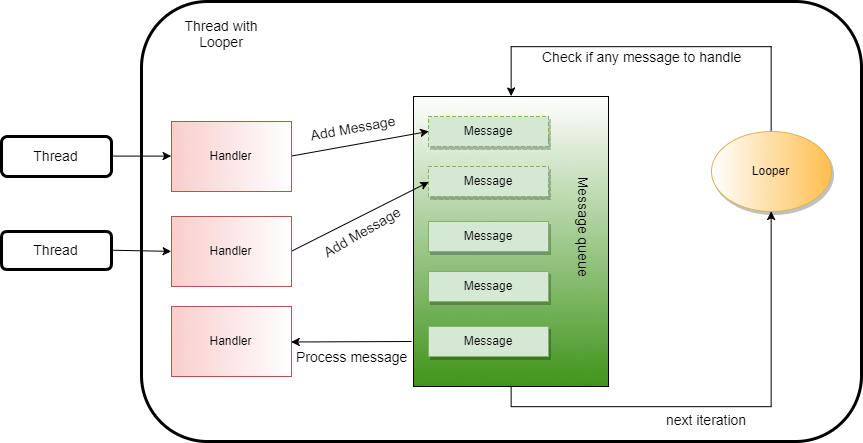
\includegraphics[scale=0.5]{looper.png}
\caption{Simple calculator}
\label{fig:simcal}
\end{figure}

A typical scenario would have a handler bound to the UI thread's Looper, being accessed from a second thread asking him to post a task to perform on the UI thread. This task would typically envolve UI updates from the second thread. This can be seen in the provided example, where upon clicking a switch we create a new thread which posts the task to disable the switch and start showing the progress bar to the UI thread. After that the new thread just waits for 5 seconds which can resemble any task taking some time and once he has finished he posts another task to the UI thread's message queue to update the UI once again. The source code can be found \href{https://github.com/JonSteinn/AndroidDevelopment/tree/master/examples/lab2/handlers}{here} and a programming session \href{https://youtu.be/__e-C97P6Eo}{here}.

\section{RxAndroid}
An Android specific binding for the RxJava library is a very powerful 3rd party option to handle background tasks. Its main components are schedulers, observers and observables. An observable can perform a background task while notifying an observer on a specified scheduler. Before we can use \href{https://github.com/ReactiveX/RxAndroid}{RxAndroid} we must add the following dependencies in our \texttt{build.gradle}.
\begin{lstlisting}[style=A_txt]
compile 'io.reactivex.rxjava2:rxandroid:2.0.1'
compile 'io.reactivex.rxjava2:rxjava:2.1.3'
\end{lstlisting}
In the provided example, we use schedulers, ovservers and observables to perform a fake time consuming task while keeping the UI thread from locking. The source code can be found \href{https://github.com/JonSteinn/AndroidDevelopment/tree/master/examples/lab2/rxandroid}{here} and a programming session \href{https://youtu.be/aSyy4MGnmQ4}{here}.

\section{Assignment - Bouncing ball}
Given a template for a view that draws graphics and a mathematical circle, your task is to make the circle move indefinitely in a diagonal direction but never leaving the screen (bouncing when colliding with its edges). You are free to use whatever threading technique you want to solve this task.

\begin{figure}[H]
\centering
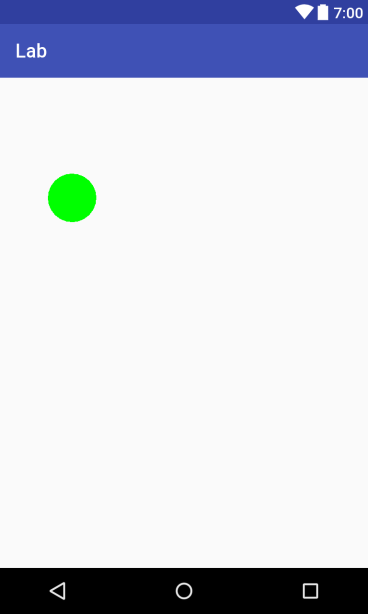
\includegraphics[scale=0.6]{bouncing_ball.png}
\caption{Bouncing ball}
\label{fig:bball}
\end{figure}

The following class should not be changed (other than the color, if you want) and you can use the \texttt{update} method to redraw the circle.
\begin{lstlisting}[style=A_Java]
public class GraphicView extends View {
    private Paint paint;
    public GraphicView(Context context, @Nullable AttributeSet attrs) {
        super(context, attrs);
        paint = new Paint();
        paint.setARGB(255, 0 /* R */, 255 /* G */, 0 /* B */);
        paint.setStyle(Paint.Style.FILL_AND_STROKE);
    }
    @Override
    public void onDraw(Canvas canvas) {
        canvas.drawCircle(
                Circle.getInstance().getX(), 
                Circle.getInstance().getY(),
                Circle.getInstance().getRadius(), 
                paint
        );
    }
    public void update() {
        this.invalidate();
    }
}
\end{lstlisting}
You are free to add what you need to the \texttt{Circle} class. It must however support accessing these 3 geometrical variables in the way that is provided.
\begin{lstlisting}[style=A_Java]
public final class Circle {
    // Geometrical variables
    private float x;
    private float y;
    public final float radius;

    // Singleton pattern
    private static final Circle INSTANCE = new Circle();
    public static Circle getInstance() {
        return INSTANCE;
    }

    // A private constructor to guarantee a single instance
    private Circle() {
        x = 100f;
        y = 100f;
        radius = 50f;
    }

    public float getX() {
        return x;
    }

    public float getY() {
        return y;
    }

    public float getRadius() {
        return radius;
    }
}
\end{lstlisting}
You can get the width and the height of the view with their \texttt{getWidth} and \texttt{getHeight} methods for the collision test. Note that the coordinate system of the canvas has the $y$ value grow downwards as is shown in figure \ref{fig:cancoord}.

\begin{figure}[H]
\centering
\begin{tikzpicture}
\draw[step=1,gray,thin,dotted] (0,-5) grid (10,0);
\draw[->] (0,0) -- (10,0);
\draw[->] (0,0) -- (0,-5);
\foreach \x in {0,1,...,9}{%
    \draw (\x,-0.1) -- (\x,0.1) node[above] {$\x$};
}
\foreach \y in {0,1,...,4}{%
    \draw (0.1,-\y) -- (-0.1,-\y) node[left] {$\y$};
}
\end{tikzpicture}
\caption{Canvas coordinate system}
\label{fig:cancoord}
\end{figure}